\section{Design Overview}
\label{sec:design}
In this section, we will elaborate on the system design for {\sys} middle-box, and how it will be deployed in a network.
A high-level end-to-end design of the system is described first, followed by the explanation for connection establishment, data transmission, and connection termination.
For simplicity, we assume there are only two middle-boxes in the network, and we have two hosts, the client and the server, willing to communicate.
The client and server are connected to middle-boxes 1 and 2, respectively.
Routing tables of end-hosts (clients and servers) define their corresponding middle-box as the gateway.
This scenario has been illustrated in Figure \ref{fig:end-to-end}.

\begin{figure}[!htbp]
    \centering
    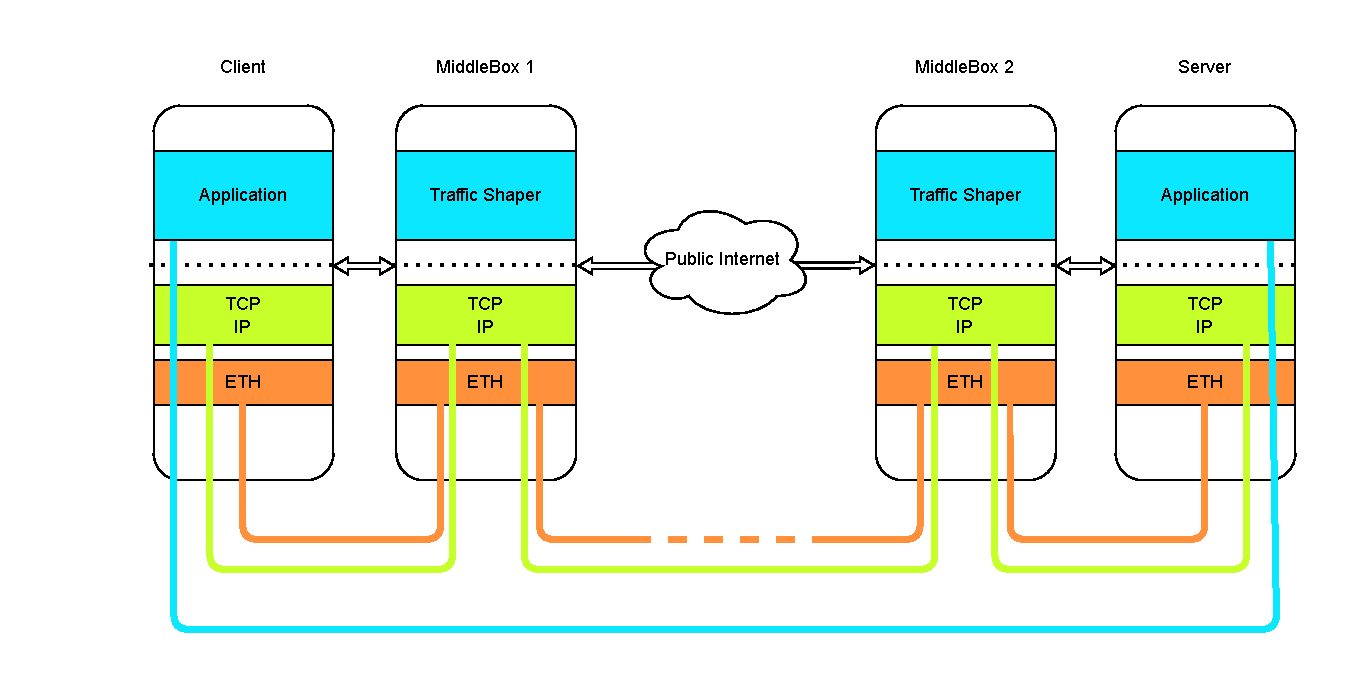
\includegraphics[width=\columnwidth]{figures/design_overview.pdf}
    \caption{End to End design of the {\sys}}
    \label{fig:end-to-end}
\end{figure}

The {\sys} middle-boxes use a reliable connection to transmit control messages.
We define six control messages between middle-boxes: \texttt{conn-req}, \texttt{conn-ack}, , \texttt{conn-est}, \texttt{term-req}, \texttt{term-ack}, and \texttt{term-est}.
Each message contains a message identifier and a flow identifier. 
The {\sys} defines the flow ID as a tuple in the following format: \texttt{flowID=<src\_ip, src\_port, dst\_ip, dst\_port, protocol>}.
In the following sections, we assume the client establishes a TCP connection to transmit data.
Therefore, the \texttt{protocol} value in the flow ID is \texttt{tcp}.
The middle-box stores flows and their states in a specific table called \textit{connection table}.

\subsection{Connection Establishment}
To establish a connection with the server, the client sends a TCP SYN packet.
The middle-box 1 intercepts the SYN packet, extract the flow identifiers, and adds a new row to the \textit{connection table} with the state "connection requested".
The middle-box 1 determines the middle-box at the receiver (middle-box 2 in our case) using the flow ID, and sends a \texttt{conn-req} control message to the middle-box 2.
Upon receiving a \texttt{conn-req} message, the middle-box 2 adds a new row to its \textit{connection table} with the "connection requested" state and uses the flow information to establish a TCP connection with the server on behalf of the client.
Once the connection with the server is acknowledged (i.e. the TCP SYN-ACK packet received from the server), middle-box 2 changes the connection to "connection acknowledged" and sends a \texttt{conn-ack} control message to the middle-box 1.
After receiving the connection acknowledgment, the middle-box 1 also changes the flow state to the "connection acknowledged". 
The middle-box 1 sends SYN-ACK packet to the client to create a connection with the client on behalf of the server.
When the connection with the client is completed, middle box 1 changes the flow state to "established" and sends a \texttt{conn-est} message to the middle-box 2.
The middle-box 2 also changes the flow state to "established" and sends an ACK message to the server.
This procedure is demonstrated in Figure \ref{fig:connection}

\begin{figure}[!htbp]
    \centering
    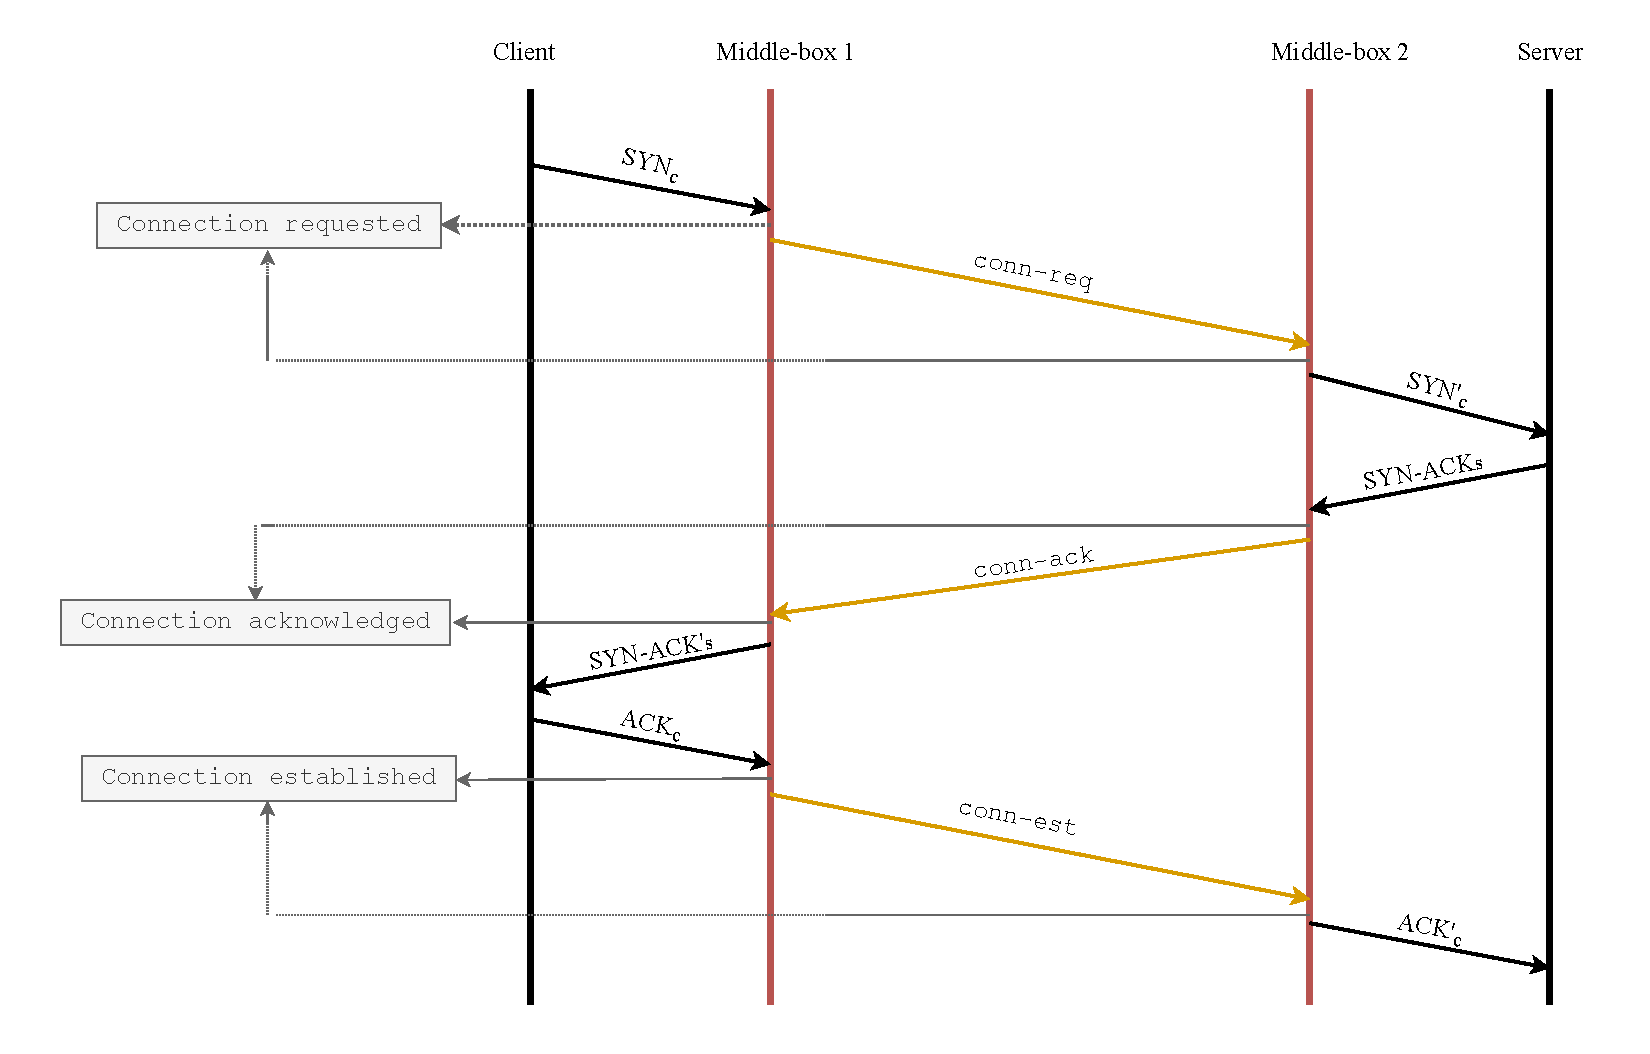
\includegraphics[width=\columnwidth]{figures/connection-establishment.pdf}
    \caption{Time line of connection establishment in {\sys}}
    \label{fig:connection}
\end{figure}
\subsection{Data Transmission}
When the connections with the client and server are established based on the procedure explained in the previous section, middle-boxes create a data channel (e.g. separate TCP connection) to transmit the shaped traffic.
At this point, three independent TCP connections are established for end-to-end traffic transmission.
For every established connection in the connection table, the middle-box creates a dedicated queue named connection private queue. 
Incoming data of the flow is stored in its corresponding queue.
The differentially private traffic shaper determines the size of data that should be moved from the flow private queue to the public queue based on the mechanism described in \ref{subsec:DP-mechanism}. 
If the determined size is larger than the amount of data in the private queue, the data will be padded with dummy data.
The padded traffic is encrypted to make the real traffic indistinguishable from the dummy data.
The middle-box on the sender side transmits the encrypted data to the middle-box on receiver side over the established data channel.
In section \ref{sec:DP-shpaing}, we elaborate on the shaping mechanism and discuss the privacy guarantees of it.
Middle-box 2 receives the encrypted traffic and enqueues it into the public queue.
Then, it decrypts the traffic, drops the dummy, and enqueues the real traffic into the public queue.
The real traffic is transmitted over the TCP connection between the middle-box 2 and the server.


\subsection{Connection Termination}
Upon receiving the TCP FIN packet from the client, the middle-box 1 changes the flow state in the \textit{connection table} to the "termination requested".
The middle-box 1 responds with TCP ACK causing the client to enter FIN\_WAIT\_1 state. 
The data transmission over the data channel between two middle-boxes continues until both private and public queues are emptied.
At this point, middle-box 1 sends a \texttt{term-req} message to the middle-box 2 on the server side.
Once the \texttt{term-req} is received by the middle-box 2, it changes the flow state to "termination requested".
Until both the public and private queues are empty, middle-box 2 continues sending data to the server.
After that, middle-box 2 sends a TCP FIN packet to the server on behalf of the client. 
When middle-box 2 receives the TCP FIN packet from the server, sends \texttt{term-ack} control message to the middle-box 1.
Upon receiving the \texttt{term-ack} message, middle-box 1 changes the flow state to "termination acknowledged" and sends the FIN packet to the client on behalf of the server.
The middle-box waits for the final TCP ACK from the client and when received changes the flow state to "terminated" and sends \texttt{term-est} to the middle-box 2.
The middle-box 2 also changes its flow state to "terminated" and sends the final TCP ACK to the server on behalf of the client, and after that, middle-box 2 terminates the data channel between 2 middle-boxes.
The procedure is represented in Figure \ref{fig:termination}.
\begin{figure}[!htbp]
    \centering
    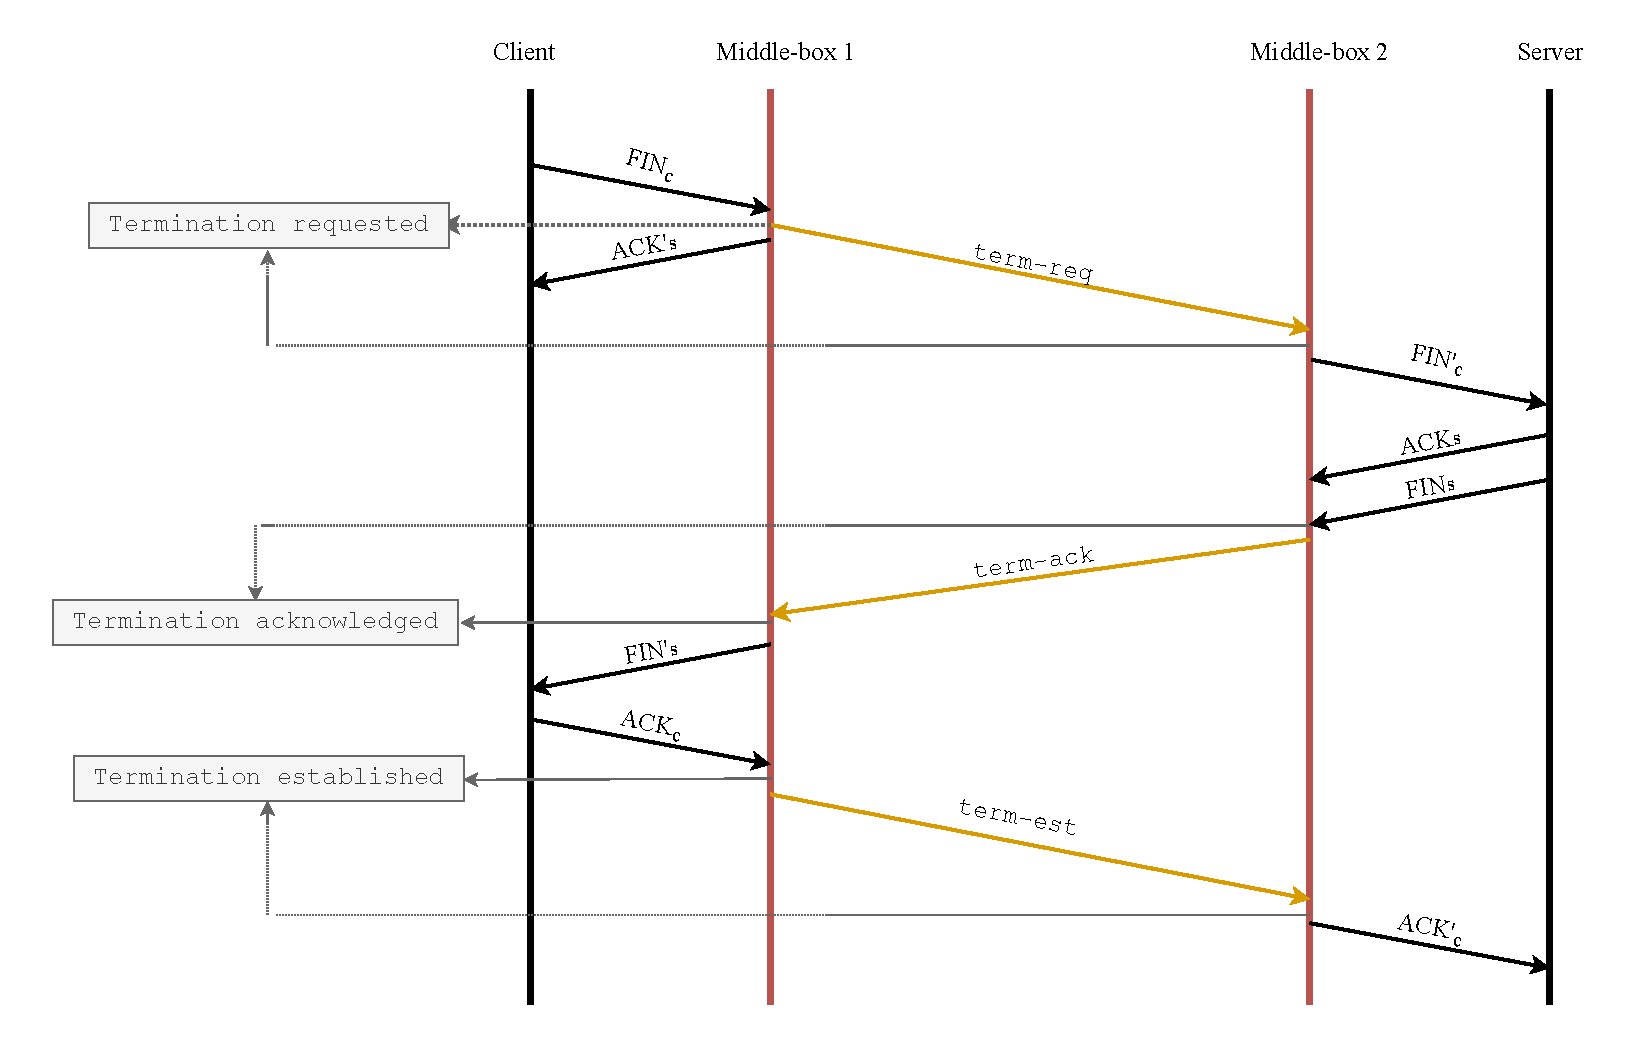
\includegraphics[width=\columnwidth]{figures/connection_termination.pdf}
    \caption{Time line of connection termination in {\sys}}
    \label{fig:termination}
\end{figure}













\begin{algorithm*}[b]
    \DontPrintSemicolon
    \SetNoFillComment
    % \KwIn{$S_N, Q, T, \varepsilon, w, D, min\_burstsize, max\_burstsize$}
    \SetKwFunction{get}{get\_DP\_size}
    \SetKwFunction{send}{send\_data}
    \SetKwProg{Fn}{Function}{:}{}

    \Fn{\get{$Q,\; \varepsilon$}}{
            $D^N = Q + LAP(\frac{D}{\varepsilon})$ \;
            $D^{N}_{clipped} =\max (B_{min}, \; \min (B_{max}, \; D_N))$ \;
            \textbf{return} $D^{N}_{clipped}$ \;
    }
    \Fn{\send{$data\_size,\; dummy\_size,\; MTU$}}{
            $buf[0:data\_size -1] =$ data\_dequeue($data\_size$)\;
            $buf[data\_size:data\_size + dummy\_size -1] =$ dummy\_dequeue($dummy\_size$)\;
            \While{$(buf.size \neq 0)$}{
                    \uIf{$(floor(buf.size/MTU) \neq 0)$}{
                            pkt.payload = $buf$.get\_data(MTU)\;
                          }
                          \Else{
                            pkt.payload = $buf$.get\_data($buf.size$)\;
                          }
                    $buf.size \mathrel{-}=$ sizeof(pkt.payload)\;
                    \tcc{Add DP header to keep track of dummy and real data.}
                    pkt.payload = add\_dp\_header(pkt.payload)\;
                    pkt.payload = encrypt(pkt.payload)\;
                    send\_udp\_pkt(pkt)\;
            }
            \textbf{return} $0$ \;
    }
    %\textbf{SendPacket}(queue\_state, pkt\_size, delay)\;
    \While{(not at end of data transmission)}{
            {sleep}($T$)\;
            $t$ = {get\_current\_time}()\;
            $Q_t$ = {get\_queue\_size}($t$)\;
            $D^S_t$ = \get($Q_t, \; \varepsilon$)\;
            \tcc{Determining the actual data we can send.}
            $D^R_t$ = $\min (Q_t, D^N_t)$\;
            \tcc{Determining the dummy data we need.}
            $D^P_t$ = $D^N_t - D^R_t$\;
            \send$(D^R_t,\; D^P_t,\; MTU)$ \;
    }
    \caption{Middle-Box Timeline}
    \label{alg:middle-box-all}
\end{algorithm*}
